\exercice{Electric field ans potentiel created by a uniformly charged ball}
\enonce{A ball of center is $O$, which radius is $R$ is uniformly charged and its total charge is $Q$.}

\enonce{The coordinates of the gradient in spherical coordinates is given : $$\vec{\grad}(f)=\frac{\partial f}{\partial r}\vec{e_r}+\frac{1}{r}\frac{\partial f}{\partial \theta}\vec{e_\theta}+\frac{1}{r\sin\theta}\frac{\partial f}{\partial \phi}\vec{e_\phi}$$}

\begin{enumerate}
  \question{Ascertain the electric field and then the electric potential in every point of space. The electric potential is taken null far away from the ball.}
    [Il faut d'abord exprimer le champ électrique puis déterminer le potentiel électrique.]
    [Effectuer les 4 étapes : analyse des invariances, analyse des symétries, choix de la surface de Gauss, théorème de Gauss.]
    [Pour exprimer la charge intérieure, il est nécessaire de distinguer les cas.]
    [Une fois le champ électrique exprimé, utiliser la relation $\vec{E}=-\vec{\text{grad}}V$ pour trouver $V$.]
    [L'analyse des symétries et des invariances permet de simplifier l'expression de $\vec{\text{grad}}V$ donnée dans l'énoncé.]
    [Déterminer d'abord la constante d'intégration dans le cas $r\gt R$ puis trouver celle dans l'autre cas par continuité de $V$ en $R$.]
    [La constante d'intégration peut être déterminée grâce au fait que $V(r)$ est nul très lion de la boule.]
  \question{Plot $E(r)$ ans $V(r)$ as a function of $r$.}
\end{enumerate}


\exercice{Champ de gravitation}
\enonce{
La masse volumique d'une planète de rayon $R=\SI{6400}{km}$ varie avec la distance $r$ au centre selon la loi $\mu(r)=\mu_0\left(1-a\left(\frac{r}{R}\right)^2\right)$. La masse volumique moyenne de la planète vaut $\mu_{\text{moy}}=\frac{m_\text{planète}}{V_\text{planète}}=\SI{5.52e3}{kg.m^{-3}}$ et celle des roches superficielles vaut $\mu(R)=\SI{2.67e3}{kg.m^{-3}}$.}

\begin{enumerate}
  \question{Calculer numériquement les valeurs de $\mu_0$ et $a$.}
    [La masse volumique de la planète et la masse volumique des roches superficielles donnent deux équations qui permettent de trouver $\mu_0$ et $a$.]
    [Comment la masse totale de la planète s'exprime-t-elle en fonction d'une intégrale de $\mu(r)$ ?]
  \question{Établir l'expression littérale du champ de gravitation créé par la planète dans tout l'espace.}
    [Effectuer les 4 étapes : analyse des invariances, analyse des symétries, choix de la surface de Gauss, théorème de Gauss.]
  \question{Pour quel rayon le champ de gravitation est-il maximal à l'intérieur de la planète ? L'exprimer en fonction de $R$.}
    [Dériver $g(r)$ pour trouver son extrémum.]
\end{enumerate} 

\exercice{Dipôle électrostatique}
\enonce{
Un dipôle est constitué d'une charge $q$ disposée au point $A$ de coordonnées carthésiennes $(a/2,0,0)$ et d'une charge $-q$ disposée au point $A'$ de coordonnées $(-a/2,0,0)$. On étudie le champ électrique et le potentiel électrique en un point $M$.On note $d$ la distance entre $A$ et $M$ et $d'$ la distance entre $A'$ et $M$. On note $r$ la distance entre $M$ et l'origine du repère.}

\enonce{
  On donne les coordonnées du gradient en coordonnées sphériques : $$\vec{\grad}(f)=\frac{\partial f}{\partial r}\vec{e_r}+\frac{1}{r}\frac{\partial f}{\partial \theta}\vec{e_\theta}+\frac{1}{r\sin\theta}\frac{\partial f}{\partial \phi}\vec{e_\phi}$$}

\begin{enumerate}
  \question{Déterminer le potentiel électrique créé par chacune des charges en fonction de $d$ et $d'$, en supposant celui-ci nul à l'infini. En déduire le potentiel électrique créé par le dipôle constitué des deux charges.}
    [Quel est le champ électrique créé par une particule ponctuelle chargée à l'origine du repère ? Quel est le potentiel électrique associé ?]
  \question{Dans l'approximation où $r>>a$, montrer que l'expression du potentiel électrique total s'écrit $$V(M)=\frac{1}{4\pi\epsilon_0r^2}\vec{d}.\vec{e_r}$$ où on exprimera $\vec{d}$. Le vecteur $\vec{d}$ est appelé moment dipolaire, à ne pas confondre avec la distance $d$.}
    [Utiliser le théorème de superposition et faire le développement limité de $V$ au premier ordre non nul.]
    [Utiliser la relation de Chasles pour relier $d$ et $d'$ à $r$.]
  \question{En déduire l'expression du champ électrique dans la même approximation.}
    [Utiliser la relation entre $v$ et $\vec{E}$ et la définition fournie du gradient en coordonnées sphériques.]
\end{enumerate}

\exercice{Condensateur cylindrique}
\enonce{
Un condensateur cylindrique est constitué de deux armatures. L'armature intérieure est un cylindre de rayon $R_1$ et de hauteur $h$, elle porte la charge $Q$ ; l'armature extérieure est un cylindre de même axe, de rayon $R_2$, de même hauteur et porte la charge $-Q$. L'espace entre les armatures est vide. On néglige les effets de bord.
}

\begin{enumerate}
  \question{Que signifie << négliger les effets de bord >> ?}
  \question{Établir l'expression du champ électrique en tout point de l'espace.}
    [Effectuer les 4 étapes : analyse des invariances, analyse des symétries, choix de la surface de Gauss, théorème de Gauss.]
  \question{Établir l'expression de la différence de potentiel entre les deux armatures.}
    [Utiliser l'expression de la circulation de $\vec{E}$ entre deux points placés sur l'un et l'autre des cylindres.]
  \question{En déduire l'expression de la capacité du condensateur cylindrique.}
\end{enumerate}

\exercice{Total Recall : Mémoires programmées}
  \begin{wrapfigure}{r}{7cm}
    \centering
    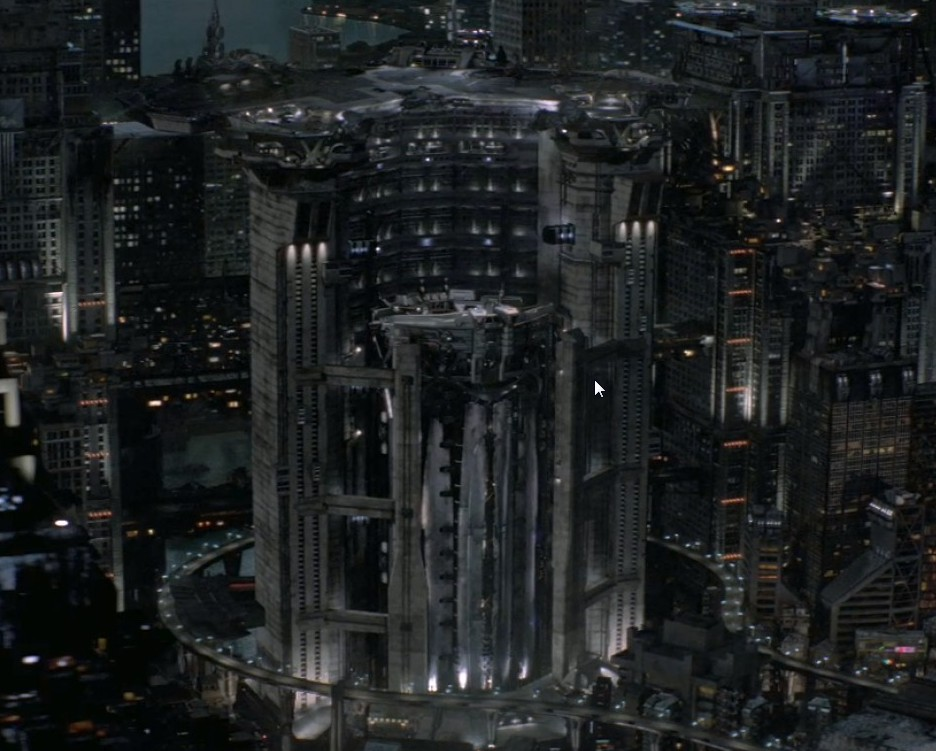
\includegraphics[width=\linewidth]{images/recall.jpg}
  \end{wrapfigure}
  \textit{Cet exercice est une résolution de problème. Il nécessite de la prise d'initiative et d'éventuelles estimations et approximations.}

  Dans le film Total Recall : Mémoires programmées (2012), les ouvriers doivent prendre quotidiennement un train gravitationnel baptisé "The Fall", qui traverse la Terre de part en part. Le train gravitationnel est mu uniquement par la gravité et tombe en chute libre jusqu'à sa destination, qu'il atteit en \SI{12}{min}.

  Données : masse de la Terre : \SI{6.0e24}{kg} ; rayon de la Terre : \SI{6400}{km}.

  \begin{enumerate}
    \item Cette durée est-elle vraisemblable ?
  \end{enumerate}

% TODO un exo avec Python

% TODO j'explique à mon cousin
